% Options for packages loaded elsewhere
\PassOptionsToPackage{unicode}{hyperref}
\PassOptionsToPackage{hyphens}{url}
%
\documentclass[
]{article}
\usepackage{lmodern}
\usepackage{amssymb,amsmath}
\usepackage{ifxetex,ifluatex}
\ifnum 0\ifxetex 1\fi\ifluatex 1\fi=0 % if pdftex
  \usepackage[T1]{fontenc}
  \usepackage[utf8]{inputenc}
  \usepackage{textcomp} % provide euro and other symbols
\else % if luatex or xetex
  \usepackage{unicode-math}
  \defaultfontfeatures{Scale=MatchLowercase}
  \defaultfontfeatures[\rmfamily]{Ligatures=TeX,Scale=1}
\fi
% Use upquote if available, for straight quotes in verbatim environments
\IfFileExists{upquote.sty}{\usepackage{upquote}}{}
\IfFileExists{microtype.sty}{% use microtype if available
  \usepackage[]{microtype}
  \UseMicrotypeSet[protrusion]{basicmath} % disable protrusion for tt fonts
}{}
\makeatletter
\@ifundefined{KOMAClassName}{% if non-KOMA class
  \IfFileExists{parskip.sty}{%
    \usepackage{parskip}
  }{% else
    \setlength{\parindent}{0pt}
    \setlength{\parskip}{6pt plus 2pt minus 1pt}}
}{% if KOMA class
  \KOMAoptions{parskip=half}}
\makeatother
\usepackage{xcolor}
\IfFileExists{xurl.sty}{\usepackage{xurl}}{} % add URL line breaks if available
\IfFileExists{bookmark.sty}{\usepackage{bookmark}}{\usepackage{hyperref}}
\hypersetup{
  hidelinks,
  pdfcreator={LaTeX via pandoc}}
\urlstyle{same} % disable monospaced font for URLs
\usepackage{color}
\usepackage{fancyvrb}
\newcommand{\VerbBar}{|}
\newcommand{\VERB}{\Verb[commandchars=\\\{\}]}
\DefineVerbatimEnvironment{Highlighting}{Verbatim}{commandchars=\\\{\}}
% Add ',fontsize=\small' for more characters per line
\usepackage{framed}
\definecolor{shadecolor}{RGB}{248,248,248}
\newenvironment{Shaded}{\begin{snugshade}}{\end{snugshade}}
\newcommand{\AlertTok}[1]{\textcolor[rgb]{0.94,0.16,0.16}{#1}}
\newcommand{\AnnotationTok}[1]{\textcolor[rgb]{0.56,0.35,0.01}{\textbf{\textit{#1}}}}
\newcommand{\AttributeTok}[1]{\textcolor[rgb]{0.77,0.63,0.00}{#1}}
\newcommand{\BaseNTok}[1]{\textcolor[rgb]{0.00,0.00,0.81}{#1}}
\newcommand{\BuiltInTok}[1]{#1}
\newcommand{\CharTok}[1]{\textcolor[rgb]{0.31,0.60,0.02}{#1}}
\newcommand{\CommentTok}[1]{\textcolor[rgb]{0.56,0.35,0.01}{\textit{#1}}}
\newcommand{\CommentVarTok}[1]{\textcolor[rgb]{0.56,0.35,0.01}{\textbf{\textit{#1}}}}
\newcommand{\ConstantTok}[1]{\textcolor[rgb]{0.00,0.00,0.00}{#1}}
\newcommand{\ControlFlowTok}[1]{\textcolor[rgb]{0.13,0.29,0.53}{\textbf{#1}}}
\newcommand{\DataTypeTok}[1]{\textcolor[rgb]{0.13,0.29,0.53}{#1}}
\newcommand{\DecValTok}[1]{\textcolor[rgb]{0.00,0.00,0.81}{#1}}
\newcommand{\DocumentationTok}[1]{\textcolor[rgb]{0.56,0.35,0.01}{\textbf{\textit{#1}}}}
\newcommand{\ErrorTok}[1]{\textcolor[rgb]{0.64,0.00,0.00}{\textbf{#1}}}
\newcommand{\ExtensionTok}[1]{#1}
\newcommand{\FloatTok}[1]{\textcolor[rgb]{0.00,0.00,0.81}{#1}}
\newcommand{\FunctionTok}[1]{\textcolor[rgb]{0.00,0.00,0.00}{#1}}
\newcommand{\ImportTok}[1]{#1}
\newcommand{\InformationTok}[1]{\textcolor[rgb]{0.56,0.35,0.01}{\textbf{\textit{#1}}}}
\newcommand{\KeywordTok}[1]{\textcolor[rgb]{0.13,0.29,0.53}{\textbf{#1}}}
\newcommand{\NormalTok}[1]{#1}
\newcommand{\OperatorTok}[1]{\textcolor[rgb]{0.81,0.36,0.00}{\textbf{#1}}}
\newcommand{\OtherTok}[1]{\textcolor[rgb]{0.56,0.35,0.01}{#1}}
\newcommand{\PreprocessorTok}[1]{\textcolor[rgb]{0.56,0.35,0.01}{\textit{#1}}}
\newcommand{\RegionMarkerTok}[1]{#1}
\newcommand{\SpecialCharTok}[1]{\textcolor[rgb]{0.00,0.00,0.00}{#1}}
\newcommand{\SpecialStringTok}[1]{\textcolor[rgb]{0.31,0.60,0.02}{#1}}
\newcommand{\StringTok}[1]{\textcolor[rgb]{0.31,0.60,0.02}{#1}}
\newcommand{\VariableTok}[1]{\textcolor[rgb]{0.00,0.00,0.00}{#1}}
\newcommand{\VerbatimStringTok}[1]{\textcolor[rgb]{0.31,0.60,0.02}{#1}}
\newcommand{\WarningTok}[1]{\textcolor[rgb]{0.56,0.35,0.01}{\textbf{\textit{#1}}}}
\usepackage{longtable,booktabs}
% Correct order of tables after \paragraph or \subparagraph
\usepackage{etoolbox}
\makeatletter
\patchcmd\longtable{\par}{\if@noskipsec\mbox{}\fi\par}{}{}
\makeatother
% Allow footnotes in longtable head/foot
\IfFileExists{footnotehyper.sty}{\usepackage{footnotehyper}}{\usepackage{footnote}}
\makesavenoteenv{longtable}
\usepackage{graphicx,grffile}
\makeatletter
\def\maxwidth{\ifdim\Gin@nat@width>\linewidth\linewidth\else\Gin@nat@width\fi}
\def\maxheight{\ifdim\Gin@nat@height>\textheight\textheight\else\Gin@nat@height\fi}
\makeatother
% Scale images if necessary, so that they will not overflow the page
% margins by default, and it is still possible to overwrite the defaults
% using explicit options in \includegraphics[width, height, ...]{}
\setkeys{Gin}{width=\maxwidth,height=\maxheight,keepaspectratio}
% Set default figure placement to htbp
\makeatletter
\def\fps@figure{htbp}
\makeatother
\setlength{\emergencystretch}{3em} % prevent overfull lines
\providecommand{\tightlist}{%
  \setlength{\itemsep}{0pt}\setlength{\parskip}{0pt}}
\setcounter{secnumdepth}{5}
\usepackage{booktabs}
\usepackage{amsthm}
\makeatletter
\def\thm@space@setup{%
  \thm@preskip=8pt plus 2pt minus 4pt
  \thm@postskip=\thm@preskip
}
\makeatother
\usepackage[]{natbib}
\bibliographystyle{plainnat}

\author{}
\date{\vspace{-2.5em}}

\begin{document}

{
\setcounter{tocdepth}{2}
\tableofcontents
}
\hypertarget{prerequisites}{%
\section{Prerequisites}\label{prerequisites}}

这份笔记主要是学习孙振球,徐勇勇老师的\textless{}\textgreater{} 第4版的过程中,尽量使用编程语言R对书中的示例进行实现的记录,
并用\href{https://github.com/rstudio/bookdown}{Bookdown}形成此文档。

如果这份文档对您有所助益,或者您对文档有疑问或建议,您可以 \textbf{\href{mailto:wxh244295043@gamil.com}{邮件}} 告知我。

建议您购买原版教材学习,您也可以在网络上找到电子书方便参考。

\begin{verbatim}
<<医学统计学>> 孙振球, 徐勇勇. 第4版[M]. 人民卫生出版社, 2014.
\end{verbatim}

\begin{center}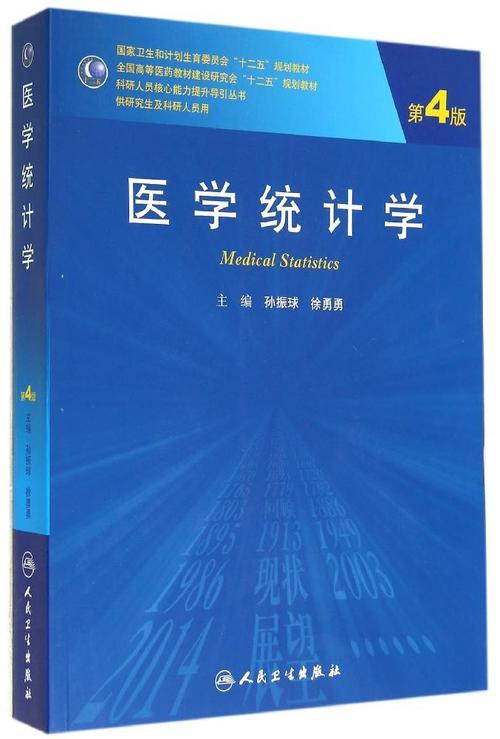
\includegraphics[width=0.25\linewidth]{image/Ms_logo} \end{center}

本文档中联系使用到的软件 \href{https://www.r-project.org/}{R} 版本是4.0.3, 和 \href{https://rstudio.com/}{RStudio},版本是 1.3.1093 .

如果您R语言的新手,您可以在下面找到一些快速学习的资料:

\begin{enumerate}
\def\labelenumi{\arabic{enumi}.}
\tightlist
\item
  \href{https://rstudio.com/resources/cheatsheets/}{RStudio Cheatsheets}
\item
  \href{https://cran.r-project.org/doc/contrib/Paradis-rdebuts_en.pdf}{R for Beginners}
\end{enumerate}

\begin{Shaded}
\begin{Highlighting}[]
\KeywordTok{sessionInfo}\NormalTok{()}
\CommentTok{## R version 4.0.3 (2020-10-10)}
\CommentTok{## Platform: x86_64-w64-mingw32/x64 (64-bit)}
\CommentTok{## Running under: Windows 10 x64 (build 19041)}

\CommentTok{## Matrix products: default}

\CommentTok{## locale:}
\CommentTok{## [1] LC_COLLATE=Chinese (Simplified)_China.936 }
\CommentTok{## [2] LC_CTYPE=Chinese (Simplified)_China.936   }
\CommentTok{## [3] LC_MONETARY=Chinese (Simplified)_China.936}
\CommentTok{## [4] LC_NUMERIC=C                              }
\CommentTok{## [5] LC_TIME=Chinese (Simplified)_China.936    }
\CommentTok{## }
\CommentTok{## attached base packages:}
\CommentTok{## [1] stats     graphics  grDevices utils     datasets  methods   base     }
\CommentTok{## }
\CommentTok{## loaded via a namespace (and not attached):}
\CommentTok{##  [1] compiler_4.0.3  bookdown_0.21   htmltools_0.5.0 tools_4.0.3    }
\CommentTok{##  [5] yaml_2.2.1      tinytex_0.27    rmarkdown_2.5   knitr_1.30     }
\CommentTok{##  [9] digest_0.6.27   xfun_0.19       rlang_0.4.8     evaluate_0.14  }
\end{Highlighting}
\end{Shaded}

\hypertarget{ux7b2cux4e8cux7ae0-ux8ba1ux91cfux8d44ux6599ux7684ux7edfux8ba1ux63cfux8ff0}{%
\section{第二章 计量资料的统计描述}\label{ux7b2cux4e8cux7ae0-ux8ba1ux91cfux8d44ux6599ux7684ux7edfux8ba1ux63cfux8ff0}}

日期: ``2020-11-13''
作者:wxhyihuan

\hypertarget{ux6d4bux8bd5ux6570ux636e}{%
\subsection{测试数据}\label{ux6d4bux8bd5ux6570ux636e}}

\begin{table}

\caption{\label{tab:tab1}某医院用随机抽样的方法检测了138名正常成年女子的红细胞数目(RBC, $*10^{12}/L$),其测量结果如下表:}
\centering
\begin{tabular}[t]{rrrrrrrrrrrr}
\toprule
V1 & V2 & V3 & V4 & V5 & V6 & V7 & V8 & V9 & V10 & V11 & V12\\
\midrule
3.96 & 4.23 & 4.42 & 3.59 & 5.12 & 4.02 & 4.32 & 3.72 & 4.76 & 4.16 & 4.61 & 4.26\\
3.77 & 4.20 & 4.36 & 3.07 & 4.89 & 3.97 & 4.28 & 3.64 & 4.66 & 4.04 & 4.55 & 4.25\\
4.63 & 3.91 & 4.41 & 3.52 & 5.03 & 4.01 & 4.30 & 4.19 & 4.75 & 4.14 & 4.57 & 4.26\\
4.56 & 3.79 & 3.89 & 4.21 & 4.95 & 3.98 & 4.29 & 3.67 & 4.69 & 4.12 & 4.56 & 4.26\\
4.66 & 4.28 & 3.83 & 4.20 & 5.24 & 4.02 & 4.33 & 3.76 & 4.81 & 4.17 & 3.96 & 3.27\\
\addlinespace
4.61 & 4.26 & 3.96 & 4.23 & 3.76 & 4.01 & 4.29 & 3.67 & 3.39 & 4.12 & 4.27 & 3.61\\
4.98 & 4.24 & 3.83 & 4.20 & 3.71 & 4.03 & 4.34 & 4.69 & 3.62 & 4.18 & 4.26 & 4.36\\
5.28 & 4.21 & 4.42 & 4.36 & 3.66 & 4.02 & 4.31 & 4.83 & 3.59 & 3.97 & 3.96 & 4.49\\
5.11 & 4.20 & 4.36 & 4.54 & 3.72 & 3.97 & 4.28 & 4.76 & 3.21 & 4.04 & 4.56 & 4.25\\
4.92 & 4.23 & 4.47 & 3.60 & 5.23 & 4.02 & 4.32 & 4.68 & 4.76 & 3.69 & 4.61 & 4.26\\
\addlinespace
3.89 & 4.21 & 4.36 & 3.42 & 5.01 & 4.01 & 4.29 & 3.68 & 4.71 & 4.13 & 4.57 & 4.26\\
4.03 & 5.46 & 4.16 & 3.64 & 4.16 & 3.76 & NA & NA & NA & NA & NA & NA\\
\bottomrule
\end{tabular}
\end{table}

\hypertarget{ux8f93ux5165ux6570ux636eux548cux9884ux5904ux7406}{%
\subsection{输入数据和预处理}\label{ux8f93ux5165ux6570ux636eux548cux9884ux5904ux7406}}

\hypertarget{ux8bfbux53d6ux6570ux636eux5e76ux5c06ux6570ux636eux8f6cux6362ux6210ux5355ux5217ux5f62ux5f0f}{%
\subsubsection{读取数据,并将数据转换成单列形式}\label{ux8bfbux53d6ux6570ux636eux5e76ux5c06ux6570ux636eux8f6cux6362ux6210ux5355ux5217ux5f62ux5f0f}}

\begin{Shaded}
\begin{Highlighting}[]
\NormalTok{RBC<-}\KeywordTok{read.table}\NormalTok{(}\StringTok{"ExampleData/02-01.txt"}\NormalTok{,}\DataTypeTok{sep=}\StringTok{"}\CharTok{\textbackslash{}t}\StringTok{"}\NormalTok{)}
\NormalTok{RBC<-}\KeywordTok{as.matrix}\NormalTok{(RBC)}
\NormalTok{RBC_q <-}\StringTok{ }\KeywordTok{c}\NormalTok{()}
\ControlFlowTok{for}\NormalTok{ (i }\ControlFlowTok{in} \KeywordTok{seq}\NormalTok{(}\DecValTok{1}\OperatorTok{:}\KeywordTok{nrow}\NormalTok{(RBC)))\{}
\NormalTok{  RBC_q <-}\StringTok{ }\KeywordTok{c}\NormalTok{(RBC_q, RBC[i,])}
\NormalTok{\}}
\NormalTok{RBC_v<-}\KeywordTok{as.vector}\NormalTok{(RBC_q)}
\NormalTok{RBC_v<-}\KeywordTok{na.omit}\NormalTok{(RBC_v)}
\end{Highlighting}
\end{Shaded}

\hypertarget{ux8ba1ux7b97ux6781ux5dee-maxminrange}{%
\subsubsection{计算极差, max()/min()/range()}\label{ux8ba1ux7b97ux6781ux5dee-maxminrange}}

\begin{Shaded}
\begin{Highlighting}[]
\CommentTok{#range(RBC_v)  #返回最小值和最大值}
\NormalTok{rge<-}\KeywordTok{max}\NormalTok{(RBC_v)}\OperatorTok{-}\KeywordTok{min}\NormalTok{(RBC_v)}
\NormalTok{rge}
\CommentTok{## [1] 2.39}
\end{Highlighting}
\end{Shaded}

\hypertarget{ux786eux5b9aux7ec4ux6bb5ux6570ux548cux7ec4ux8ddd}{%
\subsubsection{确定组段数和组距}\label{ux786eux5b9aux7ec4ux6bb5ux6570ux548cux7ec4ux8ddd}}

可以参考PAST软件中的the zero-stage rule of Wand 1997方式计算分段``最佳''个数。
\(h=3.49min(s,IQ/1.349)n^{1/3}\),其中s是样本标准差,IQ是四分位数范围。

\begin{Shaded}
\begin{Highlighting}[]
\CommentTok{#sd()计算标准差,quantile()计算分位数}
\NormalTok{s<-}\KeywordTok{sd}\NormalTok{(RBC_v)}
\CommentTok{## [1] 0.4457298}
\NormalTok{quan<-}\KeywordTok{quantile}\NormalTok{(RBC_v,}\KeywordTok{c}\NormalTok{(}\FloatTok{0.25}\NormalTok{,}\FloatTok{0.75}\NormalTok{))}
\NormalTok{iq<-quan[}\DecValTok{2}\NormalTok{]}\OperatorTok{-}\NormalTok{quan[}\DecValTok{1}\NormalTok{]}
\CommentTok{## 0.565}
\NormalTok{h<-}\FloatTok{3.49}\OperatorTok{*}\KeywordTok{min}\NormalTok{(s,iq}\OperatorTok{/}\FloatTok{1.349}\NormalTok{)}\OperatorTok{*}\NormalTok{(}\KeywordTok{length}\NormalTok{(RBC_v)}\OperatorTok{^}\NormalTok{(}\DecValTok{1}\OperatorTok{/}\DecValTok{3}\NormalTok{))}
\CommentTok{## 7.553617}
\NormalTok{h<-}\KeywordTok{ceiling}\NormalTok{(h)}
\CommentTok{## 8}
\NormalTok{i<-rge}\OperatorTok{/}\NormalTok{h}
\end{Highlighting}
\end{Shaded}

\hypertarget{ux8ba1ux7b97ux9891ux6570ux5206ux5e03}{%
\subsubsection{计算频数分布}\label{ux8ba1ux7b97ux9891ux6570ux5206ux5e03}}

根据计算的短组段数(h=8),极差值(rge=2.39))和组距(i=rge/h=0.3164)计算各组段的频数

\begin{Shaded}
\begin{Highlighting}[]
\NormalTok{breaks =}\StringTok{ }\KeywordTok{seq}\NormalTok{(}\KeywordTok{min}\NormalTok{(RBC_v), }\KeywordTok{max}\NormalTok{(RBC_v), }\DataTypeTok{length.out =} \DecValTok{8}\NormalTok{)}
\NormalTok{RBC_v.cut =}\StringTok{ }\KeywordTok{cut}\NormalTok{(RBC_v, breaks, }\DataTypeTok{right=}\NormalTok{T,}\DataTypeTok{include.lowest=}\NormalTok{T)}
\NormalTok{RBC_v.freq =}\StringTok{ }\KeywordTok{table}\NormalTok{(RBC_v.cut)}
\CommentTok{## [3.07,3.41) [3.41,3.75) [3.75,4.09) [4.09,4.44) [4.44,4.78) }
\CommentTok{##          4          17          29          51          23 }
\CommentTok{## [4.78,5.12) [5.12,5.46) }
\CommentTok{##          9           4 }
\KeywordTok{hist}\NormalTok{(RBC_v, }\DataTypeTok{right=}\OtherTok{FALSE}\NormalTok{, }
     \DataTypeTok{breaks =}\NormalTok{ breaks, }\DataTypeTok{labels =}\OtherTok{TRUE}\NormalTok{, }
     \DataTypeTok{freq =} \OtherTok{TRUE}\NormalTok{, }\DataTypeTok{col =} \StringTok{"#A8D6FF"}\NormalTok{, }
     \DataTypeTok{border =} \StringTok{"white"}\NormalTok{, }\DataTypeTok{ylim=}\KeywordTok{c}\NormalTok{(}\DecValTok{0}\NormalTok{, }\KeywordTok{max}\NormalTok{(RBC_v.freq))) }

\KeywordTok{hist}\NormalTok{(RBC_v, }\DataTypeTok{right=}\OtherTok{FALSE}\NormalTok{, }
      \DataTypeTok{breaks =}\NormalTok{ breaks, }\DataTypeTok{labels =}\OtherTok{TRUE}\NormalTok{, }
      \DataTypeTok{freq =} \OtherTok{FALSE}\NormalTok{, }\DataTypeTok{col =} \StringTok{"#A8D6FF"}\NormalTok{, }
      \DataTypeTok{border =} \StringTok{"white"}\NormalTok{, }\DataTypeTok{ylim=}\KeywordTok{c}\NormalTok{(}\DecValTok{0}\NormalTok{,}\DecValTok{1}\NormalTok{))}
\KeywordTok{lines}\NormalTok{(}\KeywordTok{density}\NormalTok{(RBC_v),}\DataTypeTok{col=}\StringTok{"red"}\NormalTok{,}\DataTypeTok{lwd=}\DecValTok{2}\NormalTok{)}
\end{Highlighting}
\end{Shaded}

\begin{figure}

{\centering 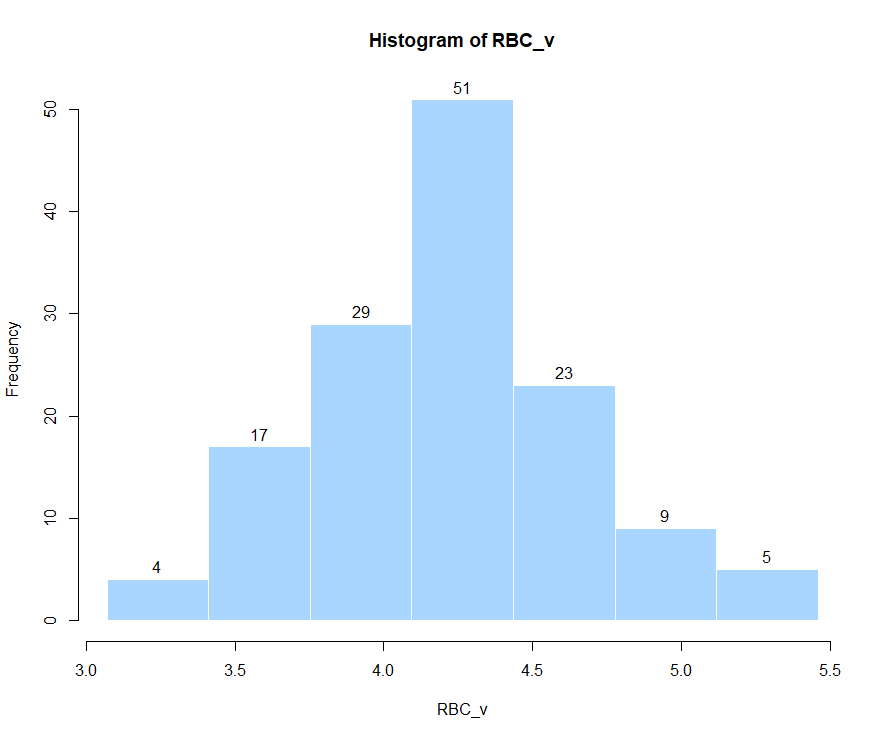
\includegraphics[width=0.49\linewidth,height=0.49\textheight]{image/a1e3904af844b14d3b57d1448690aea} 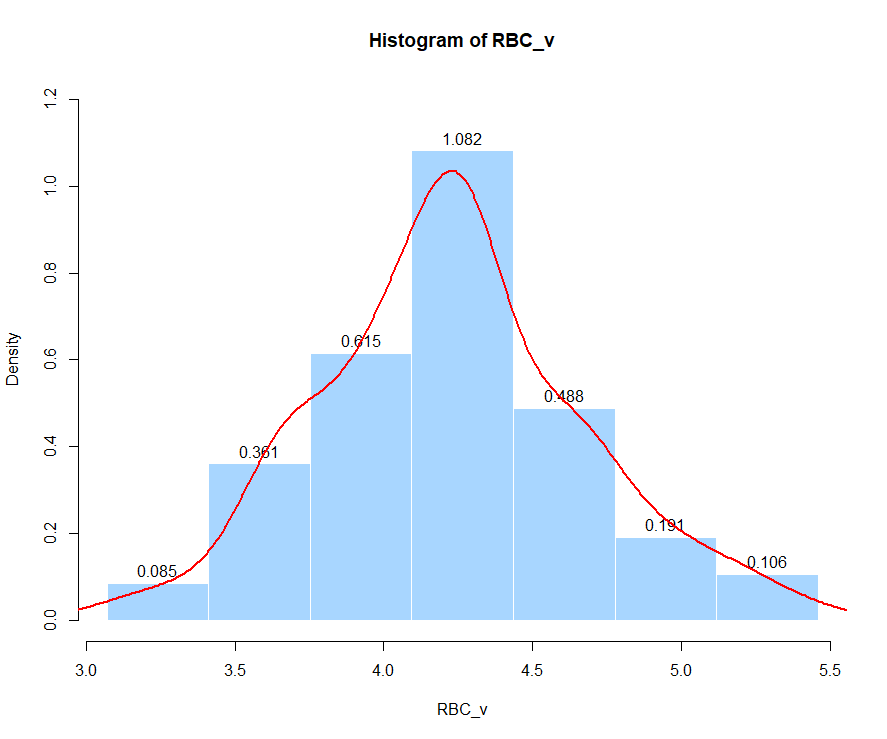
\includegraphics[width=0.49\linewidth,height=0.49\textheight]{image/5ba23e818daa7c71b147707f9b5dfd6} 

}

\caption{红细胞含量的频数分布}\label{fig:histgrah}
\end{figure}

\hypertarget{ux7edfux8ba1ux63cfux8ff0}{%
\subsection{统计描述}\label{ux7edfux8ba1ux63cfux8ff0}}

\hypertarget{ux7b97ux672fux5e73ux5747ux503c}{%
\subsubsection{算术平均值}\label{ux7b97ux672fux5e73ux5747ux503c}}

算术均数简称均数(mean),用于反映组呈对称分布的变量值在数量上的平均水平。

\begin{Shaded}
\begin{Highlighting}[]
\KeywordTok{mean}\NormalTok{(RBC_v)}
\CommentTok{## [1] 4.227029}
\end{Highlighting}
\end{Shaded}

\hypertarget{ux51e0ux4f55ux5e73ux5747ux503c}{%
\subsubsection{几何平均值}\label{ux51e0ux4f55ux5e73ux5747ux503c}}

几何均数(geometric mean)可用于反映一组经 \textbf{对数转换} 后呈对称分布的变量值在数量上的平均水平。

\begin{Shaded}
\begin{Highlighting}[]
\KeywordTok{exp}\NormalTok{(}\KeywordTok{mean}\NormalTok{(}\KeywordTok{log}\NormalTok{(RBC_v)))}
\CommentTok{## [1] 4.203676}
\end{Highlighting}
\end{Shaded}

\hypertarget{ux4e2dux4f4dux6570ux4e0eux767eux5206ux4f4dux6570}{%
\subsubsection{中位数与百分位数}\label{ux4e2dux4f4dux6570ux4e0eux767eux5206ux4f4dux6570}}

中位数(median)是将n个变量值从小到大排列,位置居于中间的那个数。当为奇数时取位次居中 的变量值,当n为偶数时取位次居中的两个变量值的均数。
它适用于各种分布类型的资料,尤其是偏态分 布资料和一端或两端无确切数值的资料。

\begin{Shaded}
\begin{Highlighting}[]
\CommentTok{#中位数(=50百分位)}
\KeywordTok{median}\NormalTok{(RBC_v)}
\KeywordTok{quantile}\NormalTok{(RBC_v,  }\FloatTok{0.5}\NormalTok{)}
\CommentTok{##  4.23}
\CommentTok{#百分位}
\KeywordTok{quantile}\NormalTok{(RBC_v, }\KeywordTok{c}\NormalTok{(}\FloatTok{0.1}\NormalTok{, }\FloatTok{0.25}\NormalTok{, }\FloatTok{0.5}\NormalTok{,}\FloatTok{0.75}\NormalTok{,}\FloatTok{0.9}\NormalTok{))}
\CommentTok{##    10%    25%    50%    75%    90% }
\CommentTok{##3.6670 3.9625 4.2300 4.5275 4.7750 }
\end{Highlighting}
\end{Shaded}

\hypertarget{ux6781ux5dee}{%
\subsubsection{极差}\label{ux6781ux5dee}}

极差即一组变量值的最大值与最小值之差。

\begin{Shaded}
\begin{Highlighting}[]
\KeywordTok{max}\NormalTok{(RBC_v)}\OperatorTok{-}\KeywordTok{min}\NormalTok{(RBC_v)}
\KeywordTok{range}\NormalTok{(RBC_v)}
\end{Highlighting}
\end{Shaded}

\hypertarget{ux56dbux5206ux4f4dux95f4ux8dddinterquartile-range}{%
\subsubsection{四分位间距(interquartile range)}\label{ux56dbux5206ux4f4dux95f4ux8dddinterquartile-range}}

四分位数(quartile)是把全部变量值分为四部分的分位数,即第1四分位数(Q .=Ps)、第2四分位数 M=P)、第3四分位数 (Qu=Ps)。 四分位数间距(quartile range)是由第3四分位数和第1四分位数相减行得,
记为 R.它般和中位数起描述偏态分们资料的分布特征

\begin{Shaded}
\begin{Highlighting}[]
\KeywordTok{IQR}\NormalTok{(RBC_v)}
\CommentTok{##  0.565}
\KeywordTok{quantile}\NormalTok{(RBC_v, }\FloatTok{0.75}\NormalTok{)}\OperatorTok{-}\KeywordTok{quantile}\NormalTok{(RBC_v, }\FloatTok{0.25}\NormalTok{)}
\CommentTok{## 0.565}
\end{Highlighting}
\end{Shaded}

\hypertarget{ux65b9ux5deeux4e0eux6807ux51c6ux5dee}{%
\subsubsection{方差与标准差}\label{ux65b9ux5deeux4e0eux6807ux51c6ux5dee}}

方差(variance)也称均方差(mean Square deviation),反映一组数据的平均离散水平。
标准差(standard deviation)是方差的正平方根,其单位与原变量值的单位相同。

\begin{Shaded}
\begin{Highlighting}[]
\KeywordTok{sd}\NormalTok{(RBC_v)}
\CommentTok{## [1] 0.4457298}
\KeywordTok{var}\NormalTok{(RBC_v)}
\CommentTok{## [1] 0.1986751}
\KeywordTok{sd}\NormalTok{(RBC_v)}\OperatorTok{^}\DecValTok{2}
\NormalTok{(}\KeywordTok{sum}\NormalTok{((RBC_v}\OperatorTok{-}\KeywordTok{mean}\NormalTok{(RBC_v))}\OperatorTok{^}\DecValTok{2}\NormalTok{))}\OperatorTok{/}\NormalTok{(}\KeywordTok{length}\NormalTok{(RBC_v)}\OperatorTok{-}\DecValTok{1}\NormalTok{)}
\CommentTok{## 0.1986751}
\end{Highlighting}
\end{Shaded}

\hypertarget{ux53d8ux5f02ux7cfbux6570}{%
\subsubsection{变异系数}\label{ux53d8ux5f02ux7cfbux6570}}

变异系数(coefficient of variation)记为CV,多用于观察指标单位不同时。

\begin{Shaded}
\begin{Highlighting}[]
\KeywordTok{sd}\NormalTok{(RBC_v)}\OperatorTok{/}\KeywordTok{mean}\NormalTok{(RBC_v)}\OperatorTok{*}\DecValTok{100}
\CommentTok{## [1] 10.54475}
\NormalTok{raster}\OperatorTok{::}\KeywordTok{cv}\NormalTok{(RBC_v)}
\CommentTok{## [1] 10.54475}
\end{Highlighting}
\end{Shaded}

\hypertarget{ux6b63ux6001ux5206ux5e03ux548cux6807ux51c6ux6b63ux6001ux5206ux5e03}{%
\subsection{正态分布和标准正态分布}\label{ux6b63ux6001ux5206ux5e03ux548cux6807ux51c6ux6b63ux6001ux5206ux5e03}}

\href{https://zh.wikipedia.org/zh-cn/\%E6\%AD\%A3\%E6\%80\%81\%E5\%88\%86\%E5\%B8\%83}{正态分布}(Normal distribution)又名高斯分布(Gaussian distribution),是一个非常常见的连续概率分布。
\textbf{正态分布}在统计学上十分重要,经常用在自然和社会科学来代表一个不明的随机变量。
可以说,弄懂正态分布是灵活运用统计学中各种假设检验方法、理解p值,均数置信区间的前提。
R包含有很丰富的正态分布相关的\href{https://stat.ethz.ch/R-manual/R-devel/library/stats/html/Normal.html}{函数功能},
比如概率密度函数dnorm(),概率累积分布函数pnorm(),正态分位函数qnorm()和用来生成特定正态分布数据序列的函数rnorm(),
以及检测数据时候符合正态分布的方法,这里主要做下面一些介绍。

\hypertarget{ux6982ux7387ux5bc6ux5ea6ux51fdux6570dnorm}{%
\subsubsection{概率密度函数dnorm()}\label{ux6982ux7387ux5bc6ux5ea6ux51fdux6570dnorm}}

\href{https://zh.wikipedia.org/zh-cn/\%E6\%A9\%9F\%E7\%8E\%87\%E5\%AF\%86\%E5\%BA\%A6\%E5\%87\%BD\%E6\%95\%B8}{概率密度函数,Probability density function},R中即为dnorm(),
它可以给出了指定均值和标准差下每个点的\textbf{概率分布的高度},
越高就代表着这个点/区间的概率越密集(大)。概率密度函数有时也被称为概率分布函数,但这种称法可能会和累积分布函数pnorm()混淆。

\begin{Shaded}
\begin{Highlighting}[]
\CommentTok{#在-10~10区间等分的 100个 数据集x}
\NormalTok{x <-}\StringTok{ }\KeywordTok{seq}\NormalTok{(}\OperatorTok{-}\DecValTok{10}\NormalTok{, }\DecValTok{10}\NormalTok{, }\DataTypeTok{by =} \FloatTok{.1}\NormalTok{)}
\CommentTok{#创建一个均值是2.5,标准差是0.5正态分布 y}
\NormalTok{y <-}\StringTok{ }\KeywordTok{dnorm}\NormalTok{(x, }\DataTypeTok{mean =} \FloatTok{2.5}\NormalTok{, }\DataTypeTok{sd =} \FloatTok{0.5}\NormalTok{)}
\CommentTok{#将 y 中的落在x数据集上的数据画出来}
\KeywordTok{plot}\NormalTok{(x,y,}\DataTypeTok{col=}\StringTok{"red"}\NormalTok{,}\DataTypeTok{pch=}\DecValTok{20}\NormalTok{)}
\end{Highlighting}
\end{Shaded}

\begin{figure}

{\centering 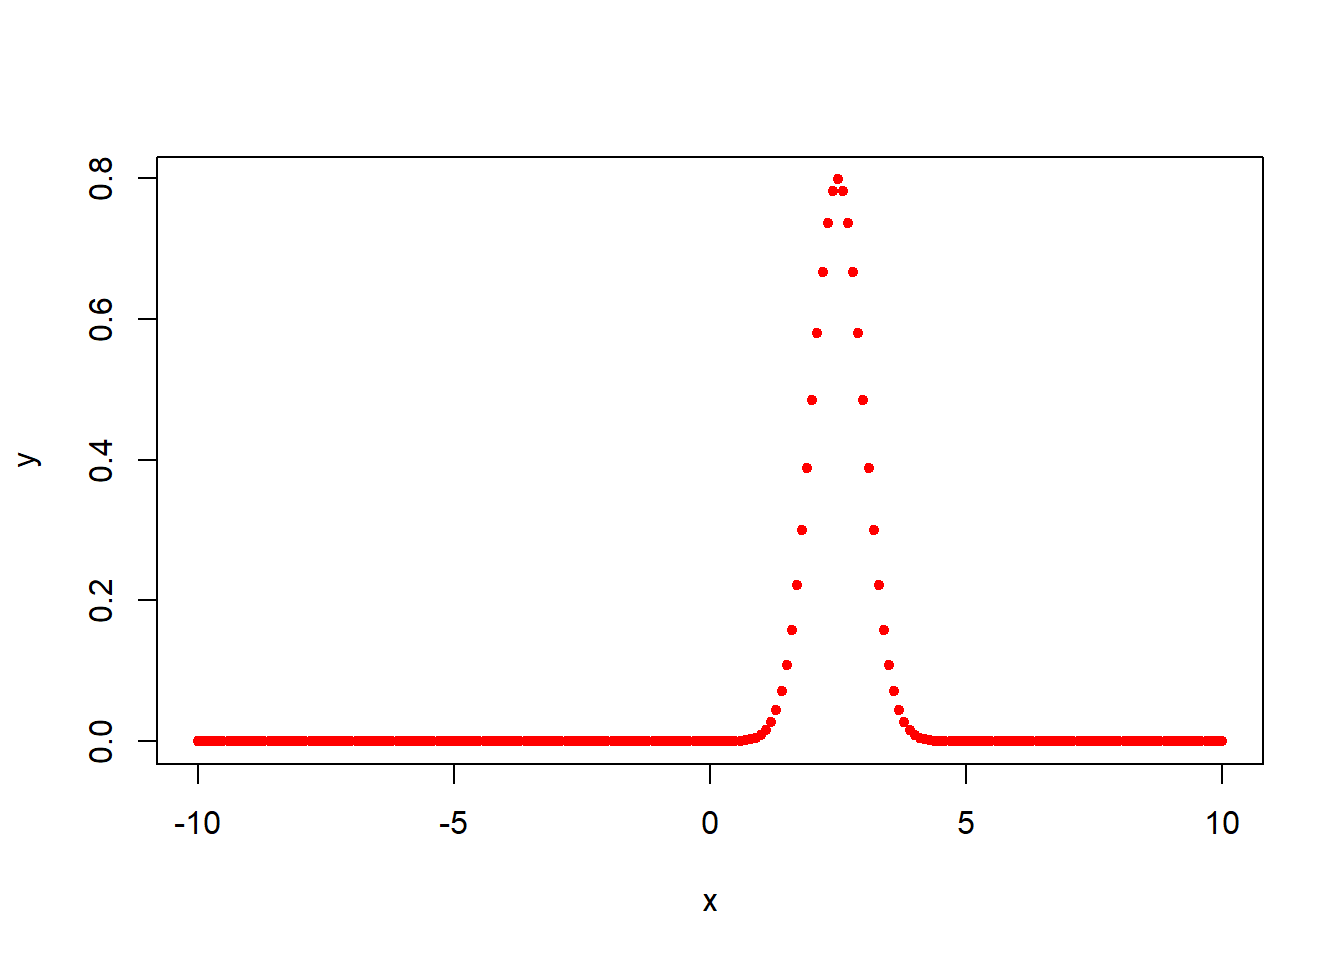
\includegraphics[width=0.49\linewidth,height=0.49\textheight]{bookdown-demo_files/figure-latex/dnorm-1} 

}

\caption{概率密度函数示例}\label{fig:dnorm}
\end{figure}

\hypertarget{ux6982ux7387ux7d2fux79efux5206ux5e03ux51fdux6570pnorm}{%
\subsubsection{概率累积分布函数pnorm()}\label{ux6982ux7387ux7d2fux79efux5206ux5e03ux51fdux6570pnorm}}

\href{https://zh.wikipedia.org/wiki/\%E7\%B4\%AF\%E7\%A7\%AF\%E5\%88\%86\%E5\%B8\%83\%E5\%87\%BD\%E6\%95\%B0}{累积分布函数,Cumulative Distribution Function},R中即为pnorm(),
又叫分布函数,是概率密度函数的积分,能完整描述一个实随机变量X的概率分布,它给出一个正态分布中小于一个给定数字的累计概率(即指定定点的左边范围的曲线面积)。

\begin{Shaded}
\begin{Highlighting}[]
\CommentTok{#在-10~10区间等分的 40个 数据集x}
\NormalTok{x <-}\StringTok{ }\KeywordTok{seq}\NormalTok{(}\OperatorTok{-}\DecValTok{10}\NormalTok{, }\DecValTok{10}\NormalTok{, }\DataTypeTok{by =} \FloatTok{.5}\NormalTok{)}
\CommentTok{#创建一个均值是2.5,标准差是0.5正态分布 y}
\NormalTok{y <-}\StringTok{ }\KeywordTok{pnorm}\NormalTok{(x, }\DataTypeTok{mean =} \FloatTok{2.5}\NormalTok{, }\DataTypeTok{sd =} \FloatTok{0.5}\NormalTok{)}
\CommentTok{#将 y 中的落在x数据集上的累计概率画出来}
\KeywordTok{plot}\NormalTok{(x,y,}\DataTypeTok{col=}\StringTok{"red"}\NormalTok{,}\DataTypeTok{pch=}\DecValTok{20}\NormalTok{)}
\end{Highlighting}
\end{Shaded}

\begin{figure}

{\centering 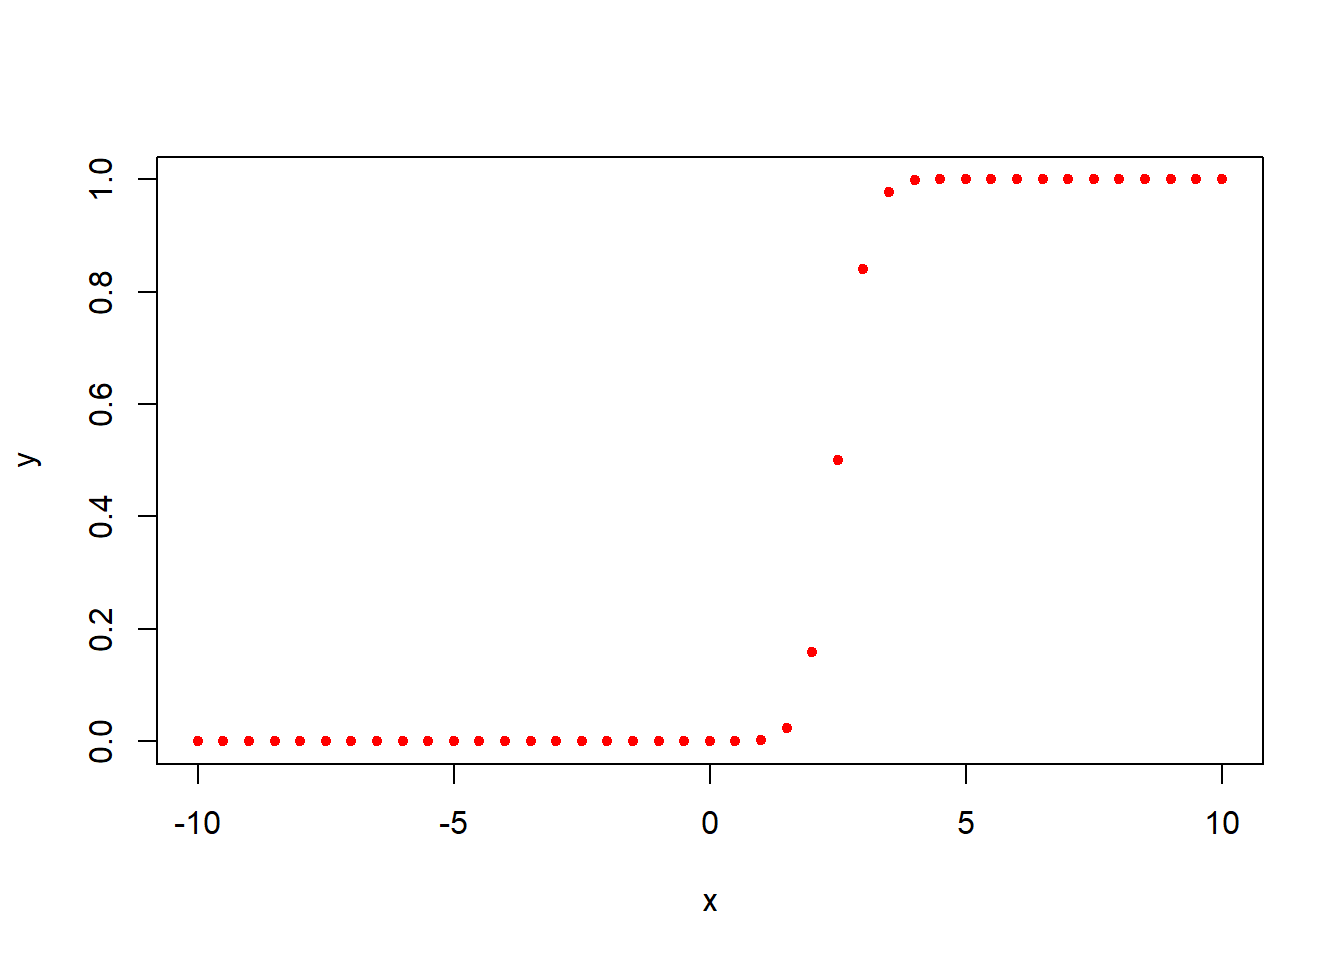
\includegraphics[width=0.49\linewidth,height=0.49\textheight]{bookdown-demo_files/figure-latex/pnorm-1} 

}

\caption{累积分布函数示例}\label{fig:pnorm}
\end{figure}

\hypertarget{ux6b63ux6001ux5206ux4f4dux51fdux6570qnorm}{%
\subsubsection{正态分位函数qnorm()}\label{ux6b63ux6001ux5206ux4f4dux51fdux6570qnorm}}

正态分位函数,R中即为qnorm(),它可以给出一个累积分布概率达到指定值的数字。

\begin{Shaded}
\begin{Highlighting}[]
\CommentTok{#在0~1区间等分的 50个 数据集x}
\NormalTok{x <-}\StringTok{ }\NormalTok{x <-}\StringTok{ }\KeywordTok{seq}\NormalTok{(}\DecValTok{0}\NormalTok{, }\DecValTok{1}\NormalTok{, }\DataTypeTok{by =} \FloatTok{0.02}\NormalTok{)}
\CommentTok{#创建一个均值是2,标准差是1正态分布 y}
\NormalTok{y <-}\StringTok{ }\KeywordTok{qnorm}\NormalTok{(x, }\DataTypeTok{mean =} \DecValTok{2}\NormalTok{, }\DataTypeTok{sd =} \DecValTok{1}\NormalTok{)}
\CommentTok{#将 y 中的落在x数据集上的数字画出来}
\KeywordTok{plot}\NormalTok{(x,y,}\DataTypeTok{col=}\StringTok{"red"}\NormalTok{,}\DataTypeTok{pch=}\DecValTok{20}\NormalTok{)}
\end{Highlighting}
\end{Shaded}

\begin{figure}

{\centering 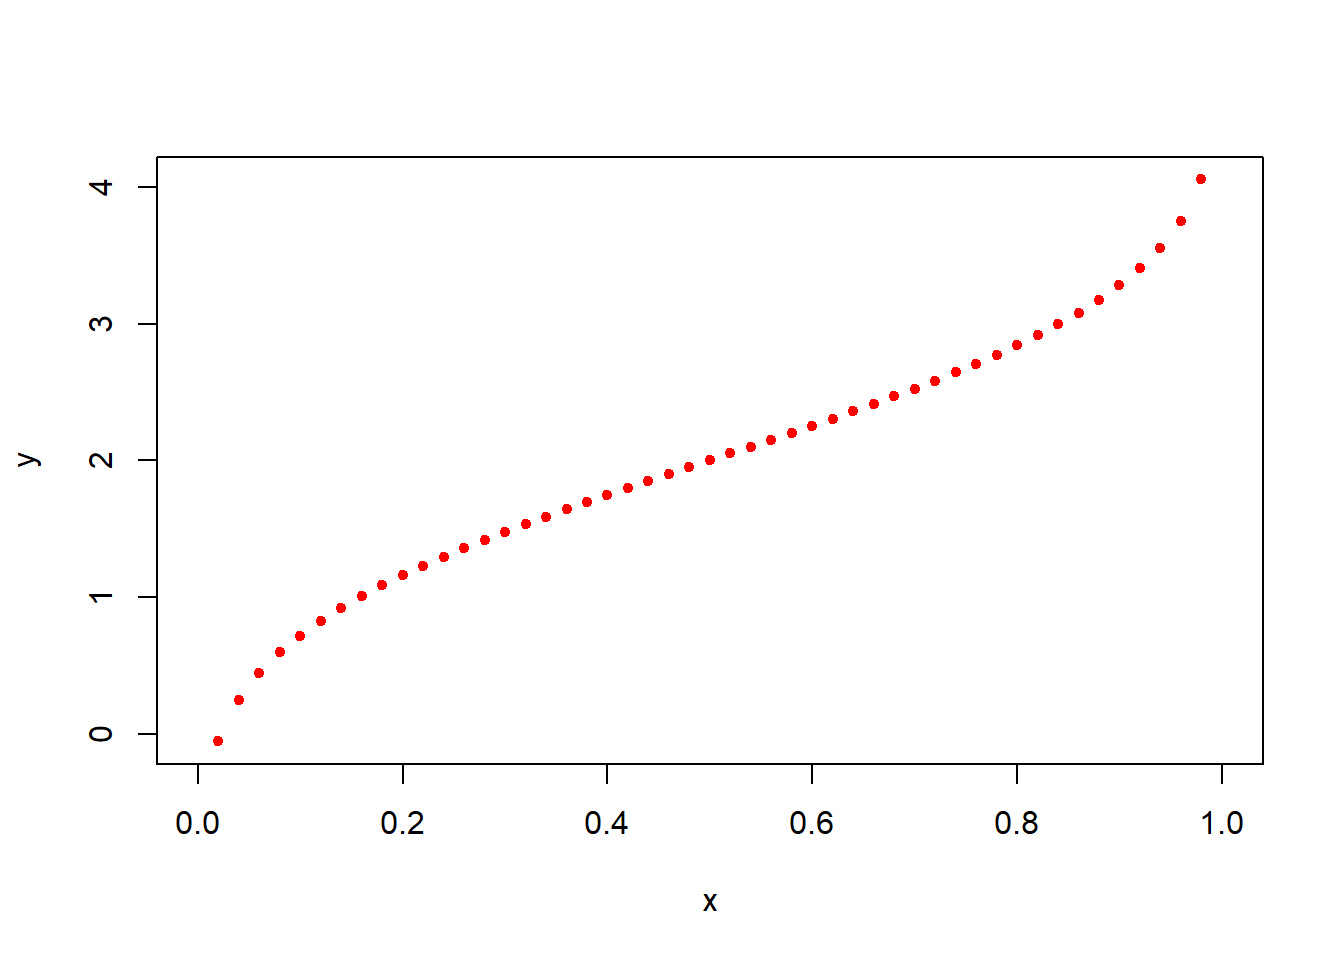
\includegraphics[width=0.49\linewidth,height=0.49\textheight]{bookdown-demo_files/figure-latex/qnorm-1} 

}

\caption{正态分位函数示例}\label{fig:qnorm}
\end{figure}

\hypertarget{ux6307ux5b9aux6b63ux6001ux5206ux4f4dux51fdux6570rnorm}{%
\subsubsection{指定正态分位函数rnorm()}\label{ux6307ux5b9aux6b63ux6001ux5206ux4f4dux51fdux6570rnorm}}

rnorm()函数用于生成符合指定均值和标准差的分布为正态分布的随机数,默认是标准正态分布,即均值为0,标准差1的正态分布。

\begin{Shaded}
\begin{Highlighting}[]
\CommentTok{#设置随机种子,便于重复后续的数据选取}
\KeywordTok{set.seed}\NormalTok{(}\DecValTok{50}\NormalTok{)}
\CommentTok{#在标准正态分布中随机选取50个数据}
\NormalTok{y <-}\StringTok{ }\KeywordTok{rnorm}\NormalTok{(}\DecValTok{50}\NormalTok{)}
\CommentTok{#对选区的数据绘制频率分布图}
\KeywordTok{hist}\NormalTok{(y,}\DataTypeTok{col=}\StringTok{"#A8D6FF"}\NormalTok{,}\DataTypeTok{labels =}\OtherTok{TRUE}\NormalTok{)}
\end{Highlighting}
\end{Shaded}

\begin{figure}

{\centering 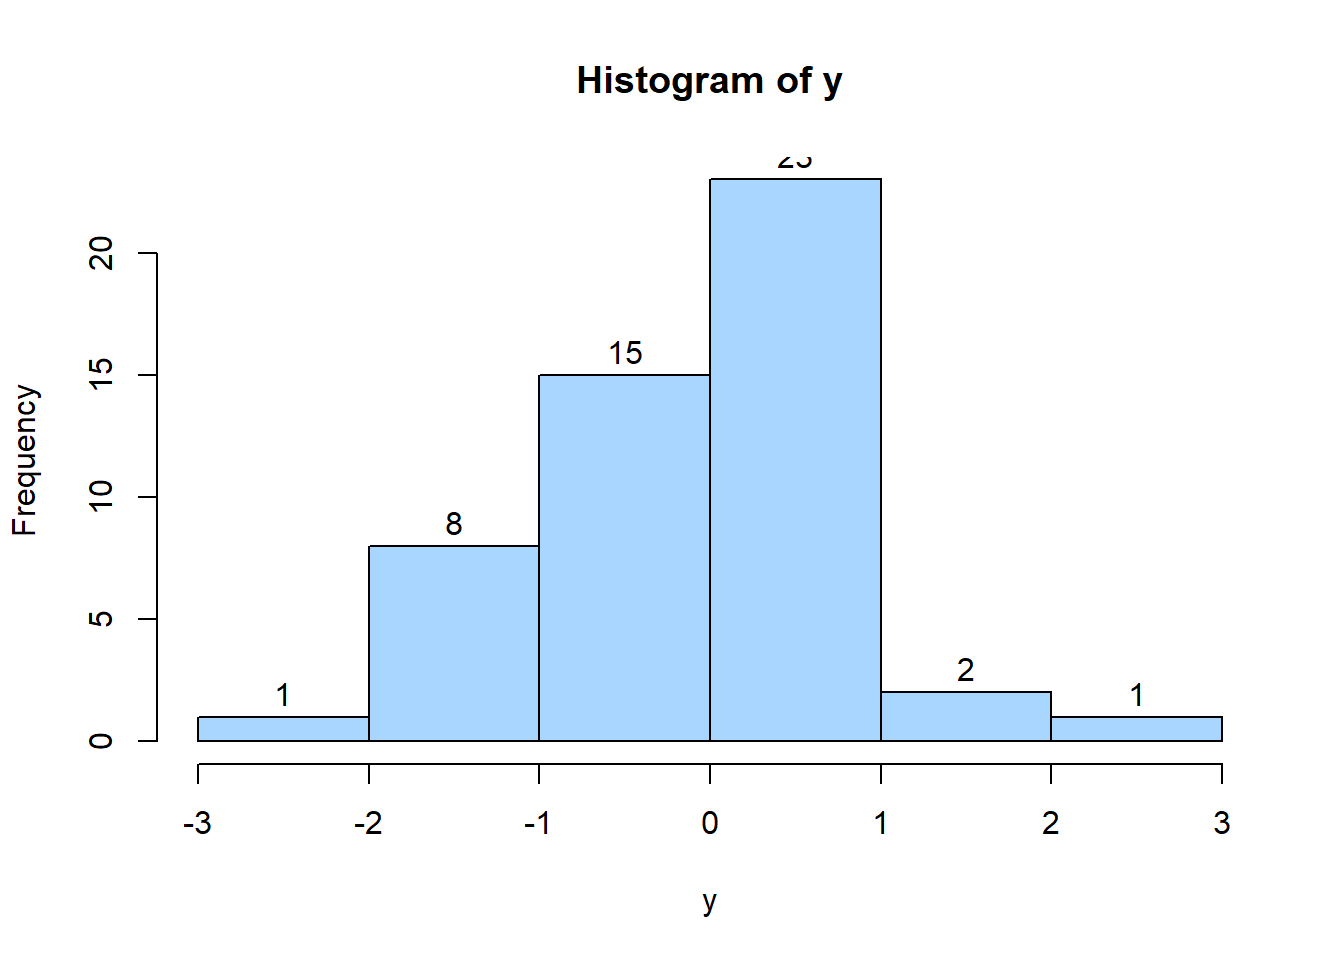
\includegraphics[width=0.49\linewidth,height=0.49\textheight]{bookdown-demo_files/figure-latex/rnorm-1} 

}

\caption{随机正态分布数据示例}\label{fig:rnorm}
\end{figure}

\hypertarget{ux6b63ux6001ux5206ux5e03ux68c0ux9a8c}{%
\subsubsection{正态分布检验}\label{ux6b63ux6001ux5206ux5e03ux68c0ux9a8c}}

许多计量资料的分析方法要求数据分布是正态或近似正态,因此对原始独立测定数据进行正态性检验是十分必要的。通过绘制数据的频数分布直方图来定性地判断数据分布正态性。

以下正态检验的资料整理自:

\begin{enumerate}
\def\labelenumi{\arabic{enumi}.}
\item
  \href{https://blog.csdn.net/u013524655/article/details/41053105?utm_medium=distribute.pc_relevant.none-task-blog-baidulandingword-7\&spm=1001.2101.3001.4242}{用R语言做正态分布检验}
\item
  \href{https://www.statsandr.com/blog/do-my-data-follow-a-normal-distribution-a-note-on-the-most-widely-used-distribution-and-how-to-test-for-normality-in-r/}{How to test the normality assumption}
\end{enumerate}

正态性检验主要有三类方法:

\begin{enumerate}
\def\labelenumi{\arabic{enumi}.}
\item
  计算综合统计量
  如动差法、夏皮罗-威尔克Shapiro-Wilk 法(W 检验) 、达戈斯提诺D′Agostino 法(D 检验) 、Shapiro-Francia 法(W′检验)。
\item
  正态分布的拟合优度检验

  如皮尔逊χ2 检验 、对数似然比检验 、柯尔莫哥洛夫Kolmogorov-Smirov 法检验。
\item
  图示法(正态概率图Normal Probability plot)

  如分位数图(Quantile Quantileplot ,简称QQ 图) 、百分位数(Percent Percent plot ,简称PP 图) 和稳定化概率图(Stablized Probability plot ,
  简称SP 图) 等。
\end{enumerate}

统计软件中常用的正态性检验方法

\begin{enumerate}
\def\labelenumi{\arabic{enumi}.}
\item
  用偏态系数和峰态系数检验数据正态性

  偏态系数Sk,它用于检验不对称性;峰态系数Ku,它用于检验峰态。 S k= 0, K u= 0 时, 分布呈正态, S k\textgreater{} 0 时, 分布呈正偏态,S k \textless{} 0 时, 分布呈负偏态。适用条件:样本含量应大于200
\item
  用夏皮罗-威尔克(Shapiro-Wilk)法检验数据正态性
  即W检验,1965 年提出,适用于样本含量n ≤50 时的正态性检;。
\item
  用达戈斯提诺(D′Agostino)法检验数据正态性
  即D检验,1971提出,正态性D检验该方法效率高,是比较精确的正态检验法。
\item
  Shapiro-Francia 法
  即W′检验,于1972 年提出,适用于50 \textless{} n \textless{} 100 时的正态性检验。
\item
  QQ图或PP图
  散点聚集在固定直线的周围,可以认为数据资料近似服从正态分布
\end{enumerate}

\textbf{常用的规则}:

\textbf{SPSS 规定}:当样本含量3 ≤n ≤5000 时,结果以Shapiro - Wilk (W 检验) 为难,当样本含量n \textgreater{} 5000 结果以Kolmogorov - Smirnov 为准。

\textbf{SAS 规定}:当样本含量n ≤2000 时,结果以Shapiro - Wilk (W 检验) 为准,当样本含量n \textgreater2000 时,结果以Kolmogorov - Smirnov (D 检验) 为准。

参考:

刘庆武,胡志艳,如何用SPSS、SAS 统计软件进行正态性检验,湘南学院学报(自然科学版),2005
朱红兵,何丽娟,在SPSS10.0 中进行数据资料正态性检验的方法,首都体育学院学报,2004

\hypertarget{ux76f4ux65b9ux56fe}{%
\paragraph{直方图}\label{ux76f4ux65b9ux56fe}}

直方图显示了分布的分布范围和形状,因此它是评估正态性的一个很好的起点。本文开始测试的红细胞浓度遵循正态曲线,因此数据似乎遵循正态分布。

\begin{Shaded}
\begin{Highlighting}[]
\KeywordTok{hist}\NormalTok{(RBC_v, }\DataTypeTok{right=}\OtherTok{FALSE}\NormalTok{, }
      \DataTypeTok{breaks =}\NormalTok{ breaks, }\DataTypeTok{labels =}\OtherTok{TRUE}\NormalTok{, }
      \DataTypeTok{freq =} \OtherTok{FALSE}\NormalTok{, }\DataTypeTok{col =} \StringTok{"#A8D6FF"}\NormalTok{, }
      \DataTypeTok{border =} \StringTok{"white"}\NormalTok{, }\DataTypeTok{ylim=}\KeywordTok{c}\NormalTok{(}\DecValTok{0}\NormalTok{,}\DecValTok{1}\NormalTok{))}

\KeywordTok{lines}\NormalTok{(}\KeywordTok{density}\NormalTok{(RBC_v),}\DataTypeTok{col=}\StringTok{"red"}\NormalTok{,}\DataTypeTok{lwd=}\DecValTok{2}\NormalTok{)}
\end{Highlighting}
\end{Shaded}

\begin{figure}

{\centering 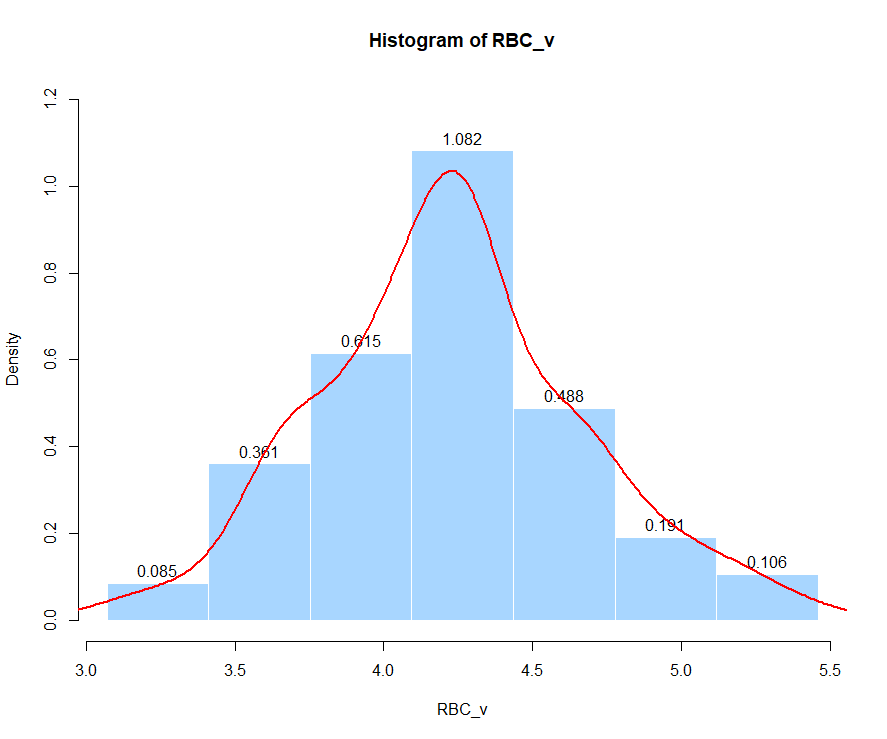
\includegraphics[width=0.49\linewidth,height=0.49\textheight]{image/5ba23e818daa7c71b147707f9b5dfd6} 

}

\caption{正态分布检验与直方图}\label{fig:histtest}
\end{figure}

\hypertarget{ux5bc6ux5ea6ux56fe}{%
\paragraph{密度图}\label{ux5bc6ux5ea6ux56fe}}

密度图提供了关于数据是否服从正态分布的直观判断。它们类似于直方图,因为它们也允许分析分布的传播和形状。但是,它们是直方图的平滑版本。

\begin{Shaded}
\begin{Highlighting}[]
\NormalTok{maintxt<-}\KeywordTok{paste}\NormalTok{(}\StringTok{"N="}\NormalTok{,}\KeywordTok{length}\NormalTok{(RBC_v),}\StringTok{","}\NormalTok{,}\StringTok{"Mean="}\NormalTok{,}\KeywordTok{round}\NormalTok{(}\KeywordTok{mean}\NormalTok{(RBC_v),}\DecValTok{3}\NormalTok{),}\StringTok{","}\NormalTok{,}\StringTok{"Sd="}\NormalTok{,}\KeywordTok{round}\NormalTok{(s,}\DecValTok{3}\NormalTok{))}
\KeywordTok{plot}\NormalTok{(}\KeywordTok{density}\NormalTok{(RBC_v),}\DataTypeTok{col=}\StringTok{"red"}\NormalTok{,}\DataTypeTok{lwd=}\DecValTok{2}\NormalTok{,}\DataTypeTok{main =}\NormalTok{ maintxt)}
\end{Highlighting}
\end{Shaded}

\begin{figure}

{\centering 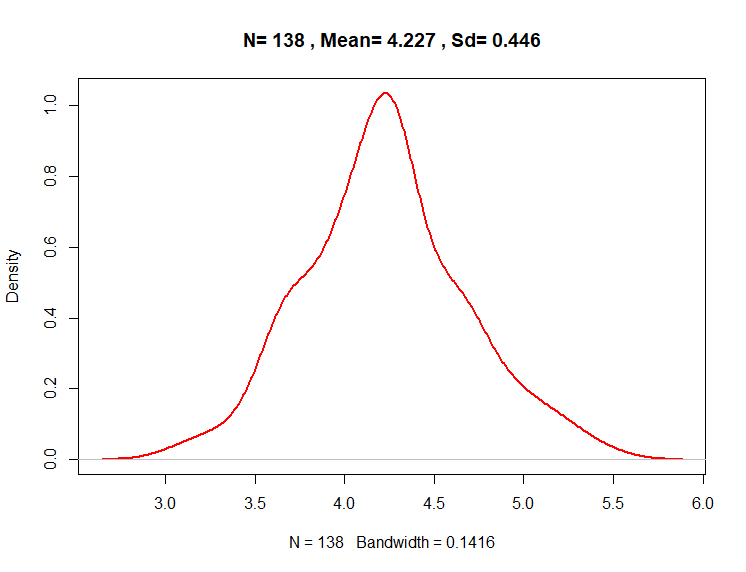
\includegraphics[width=0.49\linewidth,height=0.49\textheight]{image/Densitytest} 

}

\caption{正态分布检验与密度图}\label{fig:densitytest}
\end{figure}

\hypertarget{qq-plot}{%
\paragraph{QQ-plot}\label{qq-plot}}

有的数据从直方图和密度图很难检验正态性,因此建议用qq图来确证这些图。QQ-plot,又称正态图。在QQ-plots中,
我们只需要确定数据点是否沿着直线(有时也称为Henry's line),而不是查看数据的扩散情况(如直方图和密度图)。
如果点靠近参考线并且在置信区间内,则认为满足了正态性假设。点与参考线之间的偏差越大,偏离置信区间越远,
满足正态条件的可能性就越小。这12个成年人的身高似乎服从正态分布,因为所有的点都在置信区间内。

如果qq图所示的非正态分布(系统地偏离参考线)时,通常第一步是对数据进行对数变换,
并重新检查对数变换后的数据是否正态分布。可以应用log()函数进行对数变换。

另外,qq图也是评估回归分析的残差是否服从正态分布的一种方便的方法。

\begin{figure}

{\centering 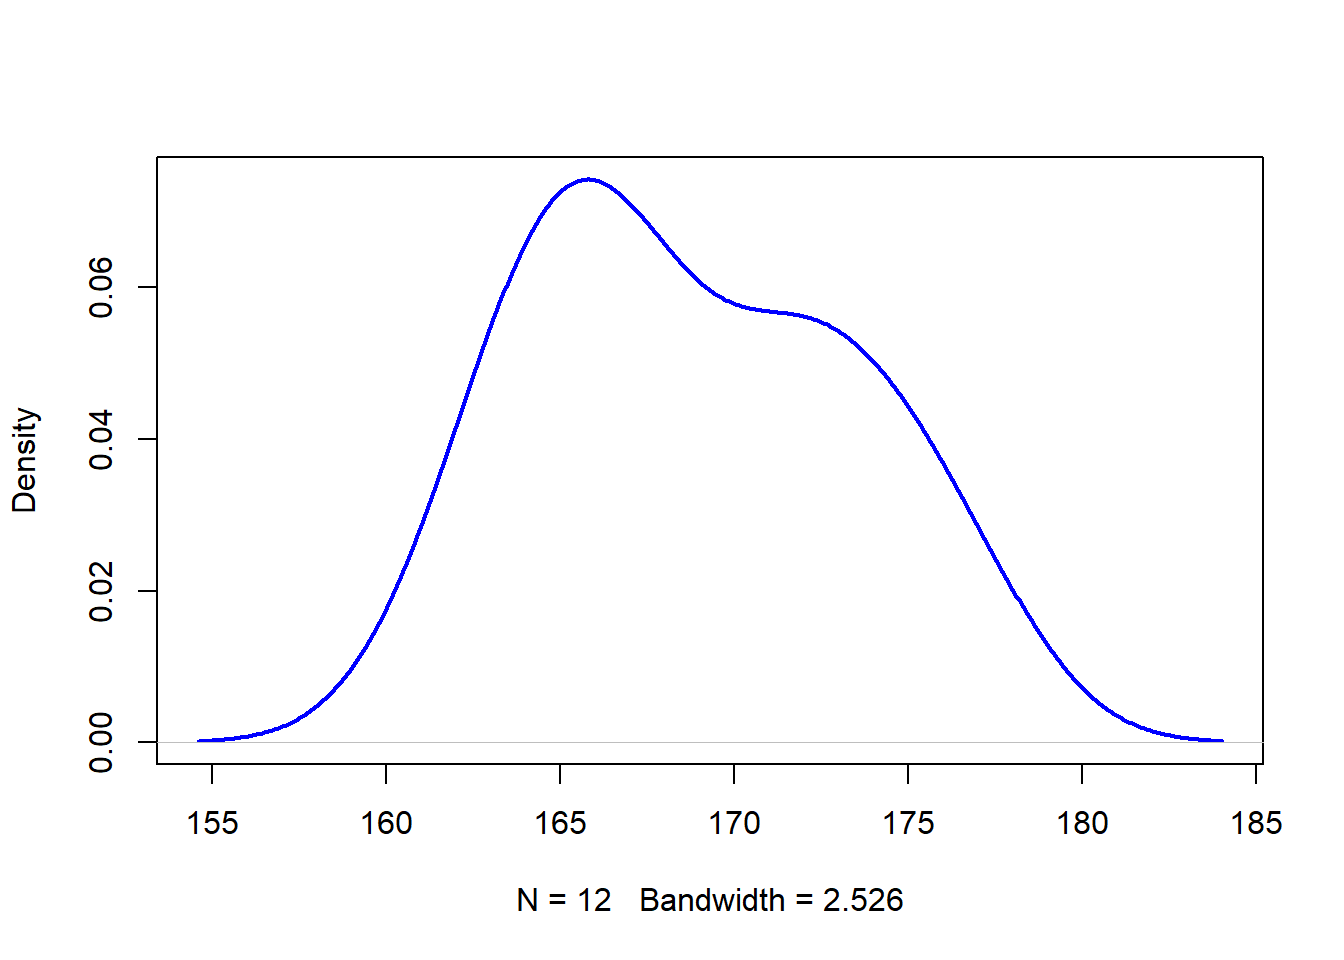
\includegraphics[width=0.49\linewidth,height=0.49\textheight]{bookdown-demo_files/figure-latex/qqplottest1-1} 

}

\caption{难以判断正态分布的密度图}\label{fig:qqplottest1}
\end{figure}

\begin{Shaded}
\begin{Highlighting}[]
\CommentTok{#qqPlot是car包中的函数,因此需要载入包}
\KeywordTok{library}\NormalTok{(car)}
\end{Highlighting}
\end{Shaded}

\begin{verbatim}
## 载入需要的程辑包:carData
\end{verbatim}

\begin{Shaded}
\begin{Highlighting}[]
\KeywordTok{set.seed}\NormalTok{(}\DecValTok{42}\NormalTok{)}
\NormalTok{dat_hist <-}\StringTok{ }\KeywordTok{data.frame}\NormalTok{( }\DataTypeTok{value =} \KeywordTok{rnorm}\NormalTok{(}\DecValTok{12}\NormalTok{, }\DataTypeTok{mean =} \DecValTok{165}\NormalTok{, }\DataTypeTok{sd =} \DecValTok{5}\NormalTok{))}
\CommentTok{##}
\KeywordTok{qqPlot}\NormalTok{(dat_hist}\OperatorTok{$}\NormalTok{value)}
\end{Highlighting}
\end{Shaded}

\begin{figure}

{\centering 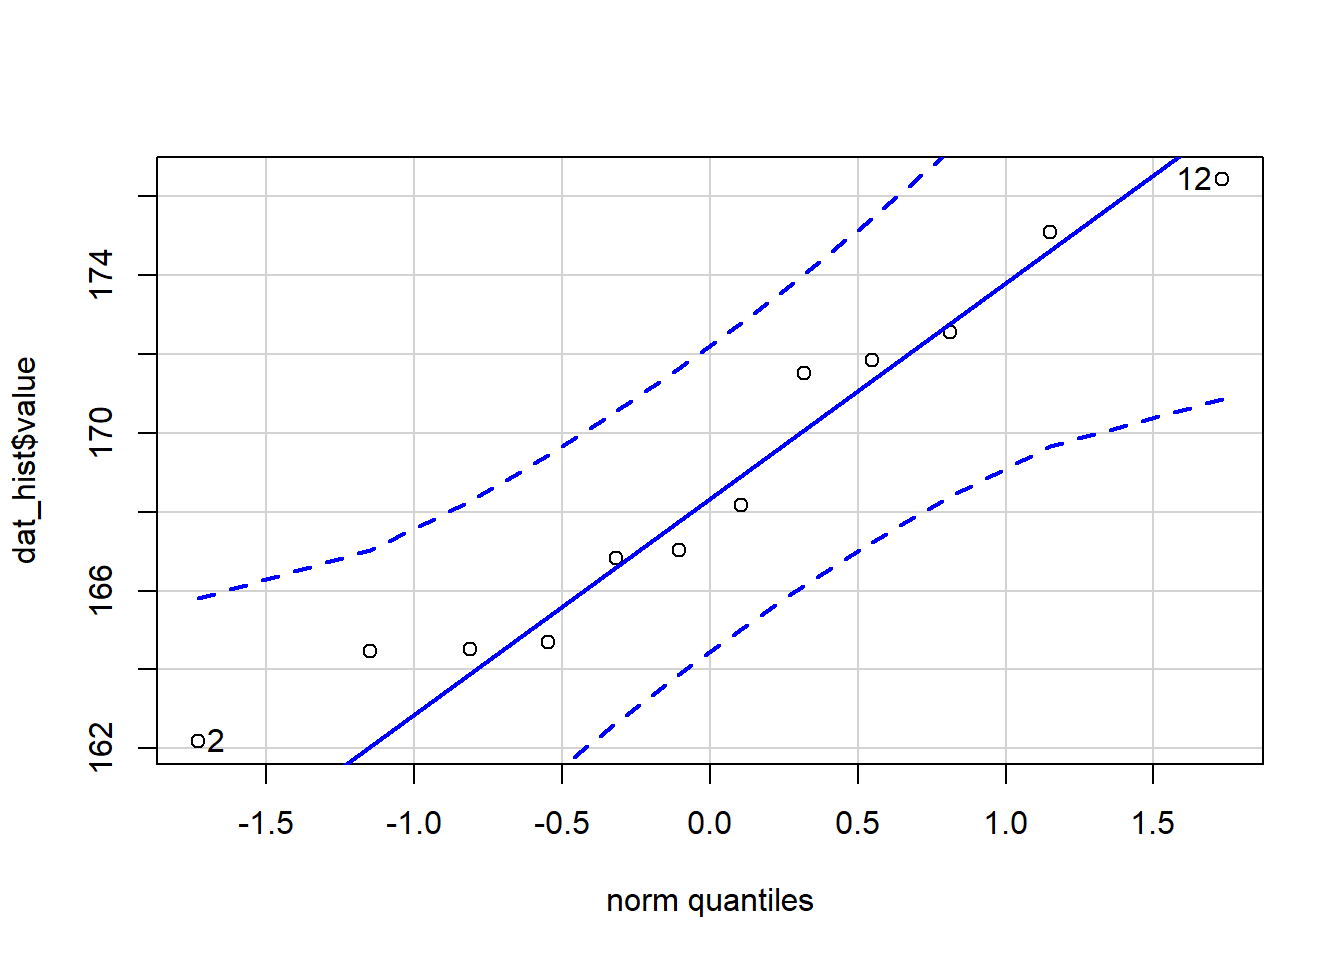
\includegraphics[width=0.49\linewidth,height=0.49\textheight]{bookdown-demo_files/figure-latex/qqplot-1} 

}

\caption{正态分布检验与QQ-plot (1)}\label{fig:qqplot}
\end{figure}

\begin{verbatim}
## [1] 12  2
\end{verbatim}

\begin{Shaded}
\begin{Highlighting}[]
\CommentTok{#qqPlot是car包中的函数,因此需要载入包}
\KeywordTok{library}\NormalTok{(car)}
\KeywordTok{qqPlot}\NormalTok{(}\KeywordTok{as.numeric}\NormalTok{(RBC_v),}\DataTypeTok{ylab=}\StringTok{"RBC"}\NormalTok{, }\DataTypeTok{main=}\StringTok{"RBC QQ-plot"}\NormalTok{)}
\end{Highlighting}
\end{Shaded}

\begin{figure}

{\centering 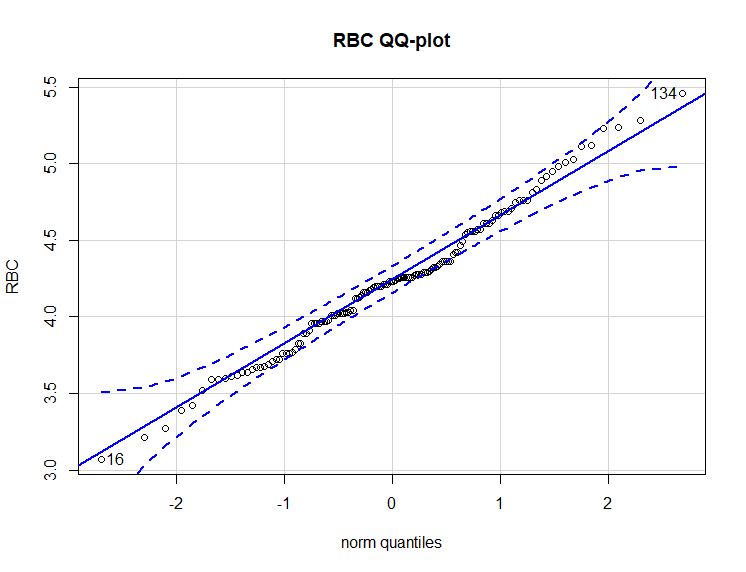
\includegraphics[width=0.49\linewidth,height=0.49\textheight]{image/qqPlot} 

}

\caption{正态分布检验与QQ-plot (2)}\label{fig:qqplot1}
\end{figure}

\hypertarget{ux6b63ux6001ux68c0ux9a8c}{%
\paragraph{正态检验}\label{ux6b63ux6001ux68c0ux9a8c}}

上述3种方法是对常态的目视检查。然而,目测有时可能不可靠,因此也有可能通过统计检验正式检验数据是否服从正态分布。
这些正态性检验将数据的分布与正态分布进行比较,以评估观察结果是否显示出偏离正态性的重要偏差。
最常用的两种正态性检验是Shapiro-Wilk检验(K检验)和Kolmogorov-Smirnov检验(D检验)。两种测试都有相同的假设,即:

\textbf{\emph{H0}} : 数据服从正态分布

\textbf{\emph{H1}} : 数据不服从正态分布

正态性检验推荐使用Shapiro-Wilk检验,因为它比Kolmogorov-Smirnov检验提供更好的效用。
在R中,正态性的Shapiro-Wilk检验可以通过函数shapiro.test()进行。

\begin{Shaded}
\begin{Highlighting}[]
\KeywordTok{set.seed}\NormalTok{(}\DecValTok{42}\NormalTok{)}
\NormalTok{dat_hist <-}\StringTok{ }\KeywordTok{data.frame}\NormalTok{( }\DataTypeTok{value =} \KeywordTok{rnorm}\NormalTok{(}\DecValTok{12}\NormalTok{, }\DataTypeTok{mean =} \DecValTok{165}\NormalTok{, }\DataTypeTok{sd =} \DecValTok{5}\NormalTok{))}
\KeywordTok{shapiro.test}\NormalTok{(dat_hist}\OperatorTok{$}\NormalTok{value)}

\CommentTok{##      Shapiro-Wilk normality test}
\CommentTok{##  }
\CommentTok{##  data:  dat_hist$value}
\CommentTok{##  W = 0.9, p-value = 0.5}
\end{Highlighting}
\end{Shaded}

从输出中,我们看到p-value\textgreater0.05意味着我们不拒绝数据服从正态分布的原假设。
该检验与qq图的方向相同,qq图与正态性没有显著偏差(因为所有点都在置信区间内)。

\begin{Shaded}
\begin{Highlighting}[]
\KeywordTok{shapiro.test}\NormalTok{(RBC_v)}

\CommentTok{##      Shapiro-Wilk normality test}
\CommentTok{##  }
\CommentTok{##  data:  as.numeric(RBC_v)}
\CommentTok{##  W = 1, p-value = 0.4}
\end{Highlighting}
\end{Shaded}

对RBC数据同样的结果。

注意的是,在实践中,正态检验通常被认为过于保守,因为对于大样本(n\textgreater50),对正态条件的一个
小偏差可能会导致违反正态判断的条件。由于正态性检验是一种假设检验,所以随着样本量的增加,其检测较小差
异的能力也会增加。因此,随着观测数的增加,Shapiro-Wilk检验变得非常敏感,甚至对正态性的一个
微小偏差也非常敏感。所以,根据正态性检验,数据不服从正态分布,尽管偏离正态分布的情况可以忽略不计,但数据
实际上服从正态分布。因此,通常情况下,正态性条件的验证是基于本文所介绍的所有方法的组合,即目视检验
(使用直方图和q-q图)和正式化检验(例如使用shapio-wilk检验)。

R中还有其他一些正态检验的方法,比如 ks.test() 函数实现Kolmogorov-Smirnov Test(D检验),
是对经验分布的拟合检验,检验的是经验分布函数和假设总体分布函数的差异,适应于大样本(n\textgreater5000)。
另外有一些package包含了丰富的检验函数,比如fBasics,nortest等。

\end{document}
